\section{The \pktlanguage compiler frontend}

We now describe the \pktlanguage compiler frontend. The compiler frontend
operates only on sequential code blocks, allowing us to borrow well-established
techniques from the compiler literature~\cite{muchnik}. However, as we show
throughout this section, constraining \pktlanguage allows us to considerably
simplify the compiler relative to compilers for general-purpose sequential
code.

\subsection{Converting to straight-line code}
A packet transaction's body can contain convoluted control flow using if-else
statements. Control flow complicates dependence analysis. We eliminate control
flow by transforming if-else statements using the C conditional operator,
starting from the innermost if statements and recursing outwards
(Figure~\ref{fig:if_convert}). This is similar to a procedure called if
conversion~\cite{allen_if_conversion}, but is much simpler because in \pktlanguage
only the if and else constructs can alter control flow 


This
transformation creates straight-line code, where control always passes from one
statement to the next without any branching. As an example, the statement



% New take at compiler:
% Middle-end: Algebric simplification, array validator, stateful_flanks, ssa, expr propagater
\label{s:compiler}

\begin{figure}
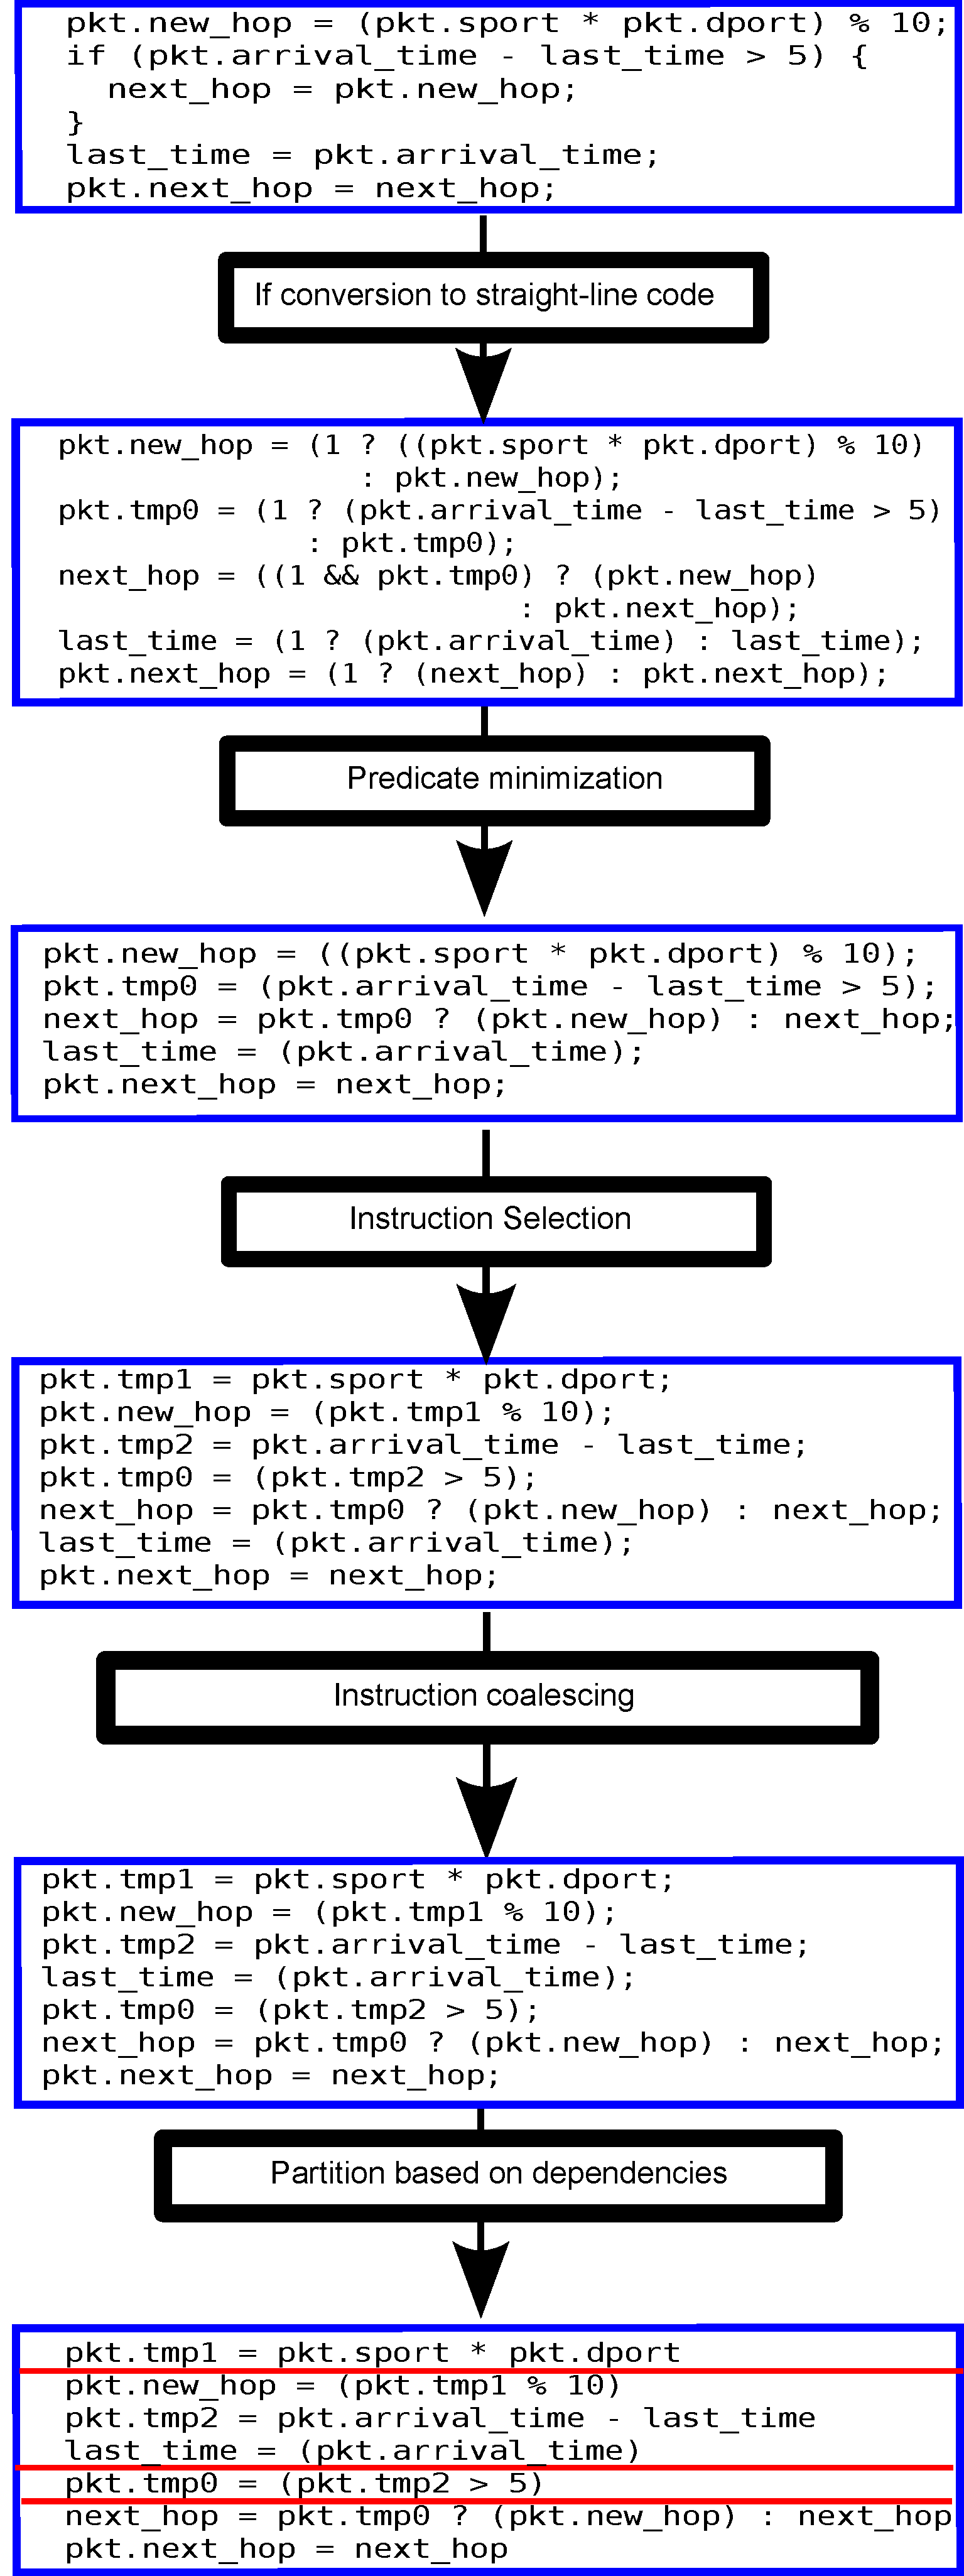
\includegraphics[width=\columnwidth]{compiler_flow.pdf}
\caption{The flow of code through the compiler}
\label{fig:flow}
\end{figure}

Figure~\ref{fig:flow} provides a high-level overview of the input and output to
the compiler for the running example that we use throughout this section: load
balancing using flowlet switching~\cite{flowlets}.  We structure the compiler
as a sequence of passes and describe each of them in turn below. 

\subsection{Predicate minimization}
Next, we simplify the predicates used in the ternary operator if possible.  In
the process, if we find the predicate is always true, we get rid of the ternary
operator altogether.

\subsection{Instruction selection}
We next replace portions of the straight-line code with equivalent code that
maps 1:1 to action primitives provided by the underlying hardware. While this
step does require knowledge of the action primitives supported by the
underlying hardware, P4 today already provides action primitives that map
1:1 to those provided by the underlying hardware, allowing us to carry out
instruction selection at the source level itself.
%Anirudh->Alvin: Ok, this is my interpretation of instruction selection
%TODO: Maybe we should just call it action primitive selection?

As a contrived example, if the underlying hardware supports read and write
operations on stateful memory, but does not support atomic increment operations
on stateful memory, we would have to replace the statement: \texttt{x = x + 1;}
with three statements:
\begin{verbatim}
int tmp1 = x;
int tmp2 = tmp1 + 1;
x = tmp2;
\end{verbatim}

Other examples of instruction selection include ``flattening''
expressions~\cite{expression_flattening} with deep ASTs into a canonical form
where the right hand side of each assignment is a simple expression that
doesn't contain any expressions within it. These simple expressions would then
map 1:1 to underlying hardware constructs.

\subsection{Instruction coalescing}

As described earlier, RMT is a shared-nothing architecture. State variables
read in a particular stage and updated downstream need recirculation to reflect
the updated value back upstream, creating a vulnerable window of packets that
can read stale state.

As far as possible, we would like to avoid recirculating packets to emulate
memory sharing across different physical stages. One way to achieve this is to
collapse instructions into the same stage using the greedy partitioning
algorithm outlined in \S\ref{ss:partitioning}. To aid our greedy partitioning
algorithm that only looks at adjacent instructions in deciding whether to
combine instructions into a stage, we first move instructions that access state
variables as close to each other as possible.

Specifically, if there are two instructions that read or write the same state
variable, we move them as close to each other as possible while respecting
Read-After-Write dependencies. This facilitates combining the instructions in
the greedy partitioning algorithm, which in turn removes the need for
recirculation.

\subsection{Partitioning based on dependencies}

At this stage, the code is correct if executed sequentially assuming exactly
one packet ever executes the code. A straightforward partitioning simply
assigns each instruction to a separate stage, but is wasteful. Many
instructions may have no dependencies between them and can be executed in
parallel.

% TODO: Anirudh->Alvin: Does this read ok?
To determine a better partitioning, we start by assigning each instruction to
its own stage. We then proceed sequentially from the first stage and grow each
stage greedily downward by merging it with the next instruction if possible.
Because instructions in a stage execute in parallel, we use the following
criterion to decide if we can execute instructions in parallel.
\begin{enumerate}
\item If there are no Read-After-Write or Write-After-Write dependencies
between a pair of instructions, it is safe to combine them.
\item If there are only Write-After-Read dependencies between instructions, we
can still combine them because the underlying hardware executes actions within
a stage simultaneously, which preserves the right semantics for
Write-After-Read dependencies.
% TODO: Only works if it fits that particular format
% (state, pkt.f) = (Guarded_Arithmetic(pkt.field, state, pkt.field), state) 

\item If there is a Read-After-Write dependency where a variable is updated in
one instruction and the updated variable needs to written into another
variable, we can still merge these instructions by replicating the same update
operation for both variables and relying on the fact that both operations
execute in parallel.
% TODO: Only works if it fits that other mold:
% (state, pkt.f) = (Guarded_Arithmetic(pkt.field, state, pkt.field), state) 
% Really, the second one is a superset of the first.
\end{enumerate}
With the above criteria, we merge a stage with the next instruction using our
greedy algorithm if the next instruction can be executed in parallel with every
instruction in the current stage. If this criteria isn't satisfied, we create a
new stage using the next instruction and proceed greedily again until we have
covered all instructions.

%%%\subsection{Detecting memory sharing across stages}
%%%In our entire discussion so far, we make no distinction between stateful
%%%variables and packet-local variables. This is because, if there is only a
%%%single packet in the system, there is no distinction between the two.
%%%
%%%In this pass, we scan the partitioning looking for stateful variables (any
%%%globally declared variable), and checking if any stateful variable is read in
%%%one stage and then written in a subsequent stage. If this is the case, that
%%%stateful variable needs to be shared across stages and the best we can do is to
%%%approximately emulate such sharing using recirculation.
%%%
%%%Instead, if a stateful variable is written in exactly one stage, but read in
%%%multiple stages following the stage that it is written in, we can achieve this
%%%effect by simply writing the stateful variable into a packet field that then
%%%carries the value to subsequent stages.
%%%
%%%We note here that this pass relies on the instruction selection pass to
%%%determine a good set of instructions that map closely to the hardware. For
%%%instance, if instruction selection cannot rewrite the set of sequential
%%%statements: \texttt{x = x + y; y = y + x;} into the tupled form \texttt{(x, y)
%%%= (x + y, 2 * y + x);}, then the one-packet compiler will move \texttt{y = y +
%%%x;} into the stage following \texttt{x = x + y;} causing spurious memory
%%%sharing.
%%%

%%%\subsection{Patching code to achieve memory sharing}
%%%\label{ss:patching}
%%%The previous pass might detemine that a stateful variable needs to be shared
%%%across stages, because it is read in one and written in a stage downstream. If
%%%this is the case, we need to clone a packet and recirculate back to the first
%%%stage of the pipeline that it needs to be read in.
%%%
%%%Because the pipeline needs to keep up with line rate and cannot be paused, we
%%%the implementation needs to handle both new data packets and recirculated
%%%cloned packets that carry state updates. We achieve this by patching the code
%%%created by the previous pass to execute the algorithm on batches of packets
%%%instead rather than every packet. We outline the patching procedure below.
%%%
%%%The first stage maintains a state variable $in\_progress$ to denote whether the
%%%algorithm is currently being executed or not. When the first data packet is
%%%received, it set $in\_progress$ to true, executes whatever other operations
%%%need to be executed as part of the algorithm itself, and passes the packet
%%%downstream to other stages with an $execute\_algorithm$ field set in the
%%%packet. The remaining stages simply follow the lead of the first stage and
%%%execute the algorithm if the $execute\_algorithm$ field is set, accumulating
%%%writes to shared variables in packet fields. At the end of the last stage, we
%%%clone a packet containing all these writes and recirculate it back into the
%%%pipeline to update all state variables. Once all state is updated, we
%%%recirculate the cloned packet a second time to reset the $in\_progress$ bit to
%%%false again.
%%%
%%%We are still left with the question of what to do when $in\_progress$ is true
%%%and a new data packet is received in the pipeline. For now, we simply pass
%%%these packets through unchanged, although there are likely other alternatives.
%%%This pass-through mode corresponds roughly to transactional semantics on
%%%batches of packets, where the batch size is the number of packets that arrive
%%%during the time it takes to recirculate a packet twice. While this may not be a
%%%reasonable solution for all data-plane algorithms, some meausrement algorithms
%%%can work on a sampled stream of packets with graceful performance degradation.
%%%We evaluate this performance degradation quantitatively in
%%%\S\ref{ss:evaluation_approx}, leaving a more accurate characterization of possible
%%%approximations to future work.

%%%\subsection{Translating to P4}
%%%As a final step, we translate the partitioned code (patched, if required)
%%%into P4. This is a conceptually straightforward process:
%%%\begin{enumerate}
%%%\item We add newly created temporary variables to the header and parser
%%%specifications so that P4 can automatically generate the parser state machine.
%%%\item We create a P4 logical table for each partition.
%%%\item The set of packets on which the algorithm will run is specified using
%%%an appropriate match type (exact, ternary, or longest-prefix) on specific
%%%header fields within each logical table.
%%%\item We create a P4 action in each logical table from the code in the
%%%corresponding partition.
%%%\item Lastly, the control-flow between P4 tables mirrors the order of
%%%partitions.
%%%\end{enumerate}

%Advanced idioms:
%--> Pipeline wide memory using recirculation primitive.
%--> Tupled Stateful operations: <x, y> <--- f(x, y).
%--> Multiply accumulate (MAC).
%
